
%place your content here, feel free to create subcontent files
\begin{block}{\blocktitle{Experimental Setup}}
\begin{center}
\raisebox{0.75cm}{
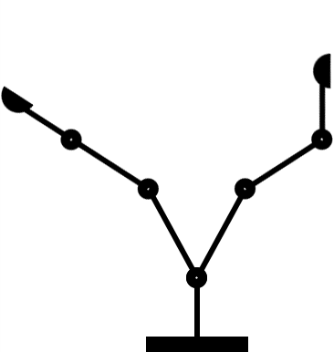
\includegraphics[width=.2\columnwidth]{pics/throw}}
\hspace*{1cm}
%\includegraphics[width=.35\columnwidth]{pics/xy_scatter_color_tau}
\hspace*{1cm}
%\includegraphics[width=.35\columnwidth]{pics/xy_scatter_color_g0}
\begin{itemize}
 \item Ball-throwing in simulation of COMPI arm (\url{github.com/rock-simulation/mars})
 \item Contexts chosen from target area: $[1, 2.5]m \times [-1, 1]m$
 \item Manually initialized joint-space DMP such that a fixed target position is hit
 \item Adapt to new target by modifying meta-parameters (execution time $\tau$ and angle of first joint $g_0$); $\tau \in [0.2, 5]$ and $g_0 \in \left[-\frac{\pi}{2}, \frac{\pi}{2}\right]$
 \item $R(s, \theta) = -\vert\vert s - b_s(\theta) \vert\vert_2^2 - 0.01\sum_t v_t^2$
 \begin{itemize}
   \item $b_s(\theta)$:  position hit for parameters $\theta$; $v_t$: joint velocities at time $t$
 \end{itemize}
 \item Deterministic affine upper-level policy; trained with C-REPS \cite{kupcsik_data-efficient_2013} update on all samples
\end{itemize}
\end{center}
\end{block}

\begin{block}{\blocktitle{Results}}
\begin{center}
\begin{itemize}
 \item Comparison of different approaches for exploration
 \begin{enumerate}
  \item Active contextual entropy search ($N_{nn} = 20$ and $N_{nn} = 1$)
  \item BO-CPS + Entropy Search +  random context selection
  \item BO-CPS + GP-UCB with $\kappa=5.0$ (``pure exploration'') + random context selection
  \item Random parameter and context selection
 \end{enumerate}
 \item Entropy Search outperforms GP-UCB because UCB aggressively samples parameters at the boundaries (high uncertainty but low global information)
 \item ACES outperforms random context selection, in particular when $N_{nn} = 20$
 \item ACES\_20 tends to avoid performing trials at the boundaries of the context space
\end{itemize}

\begin{figure}
\centering
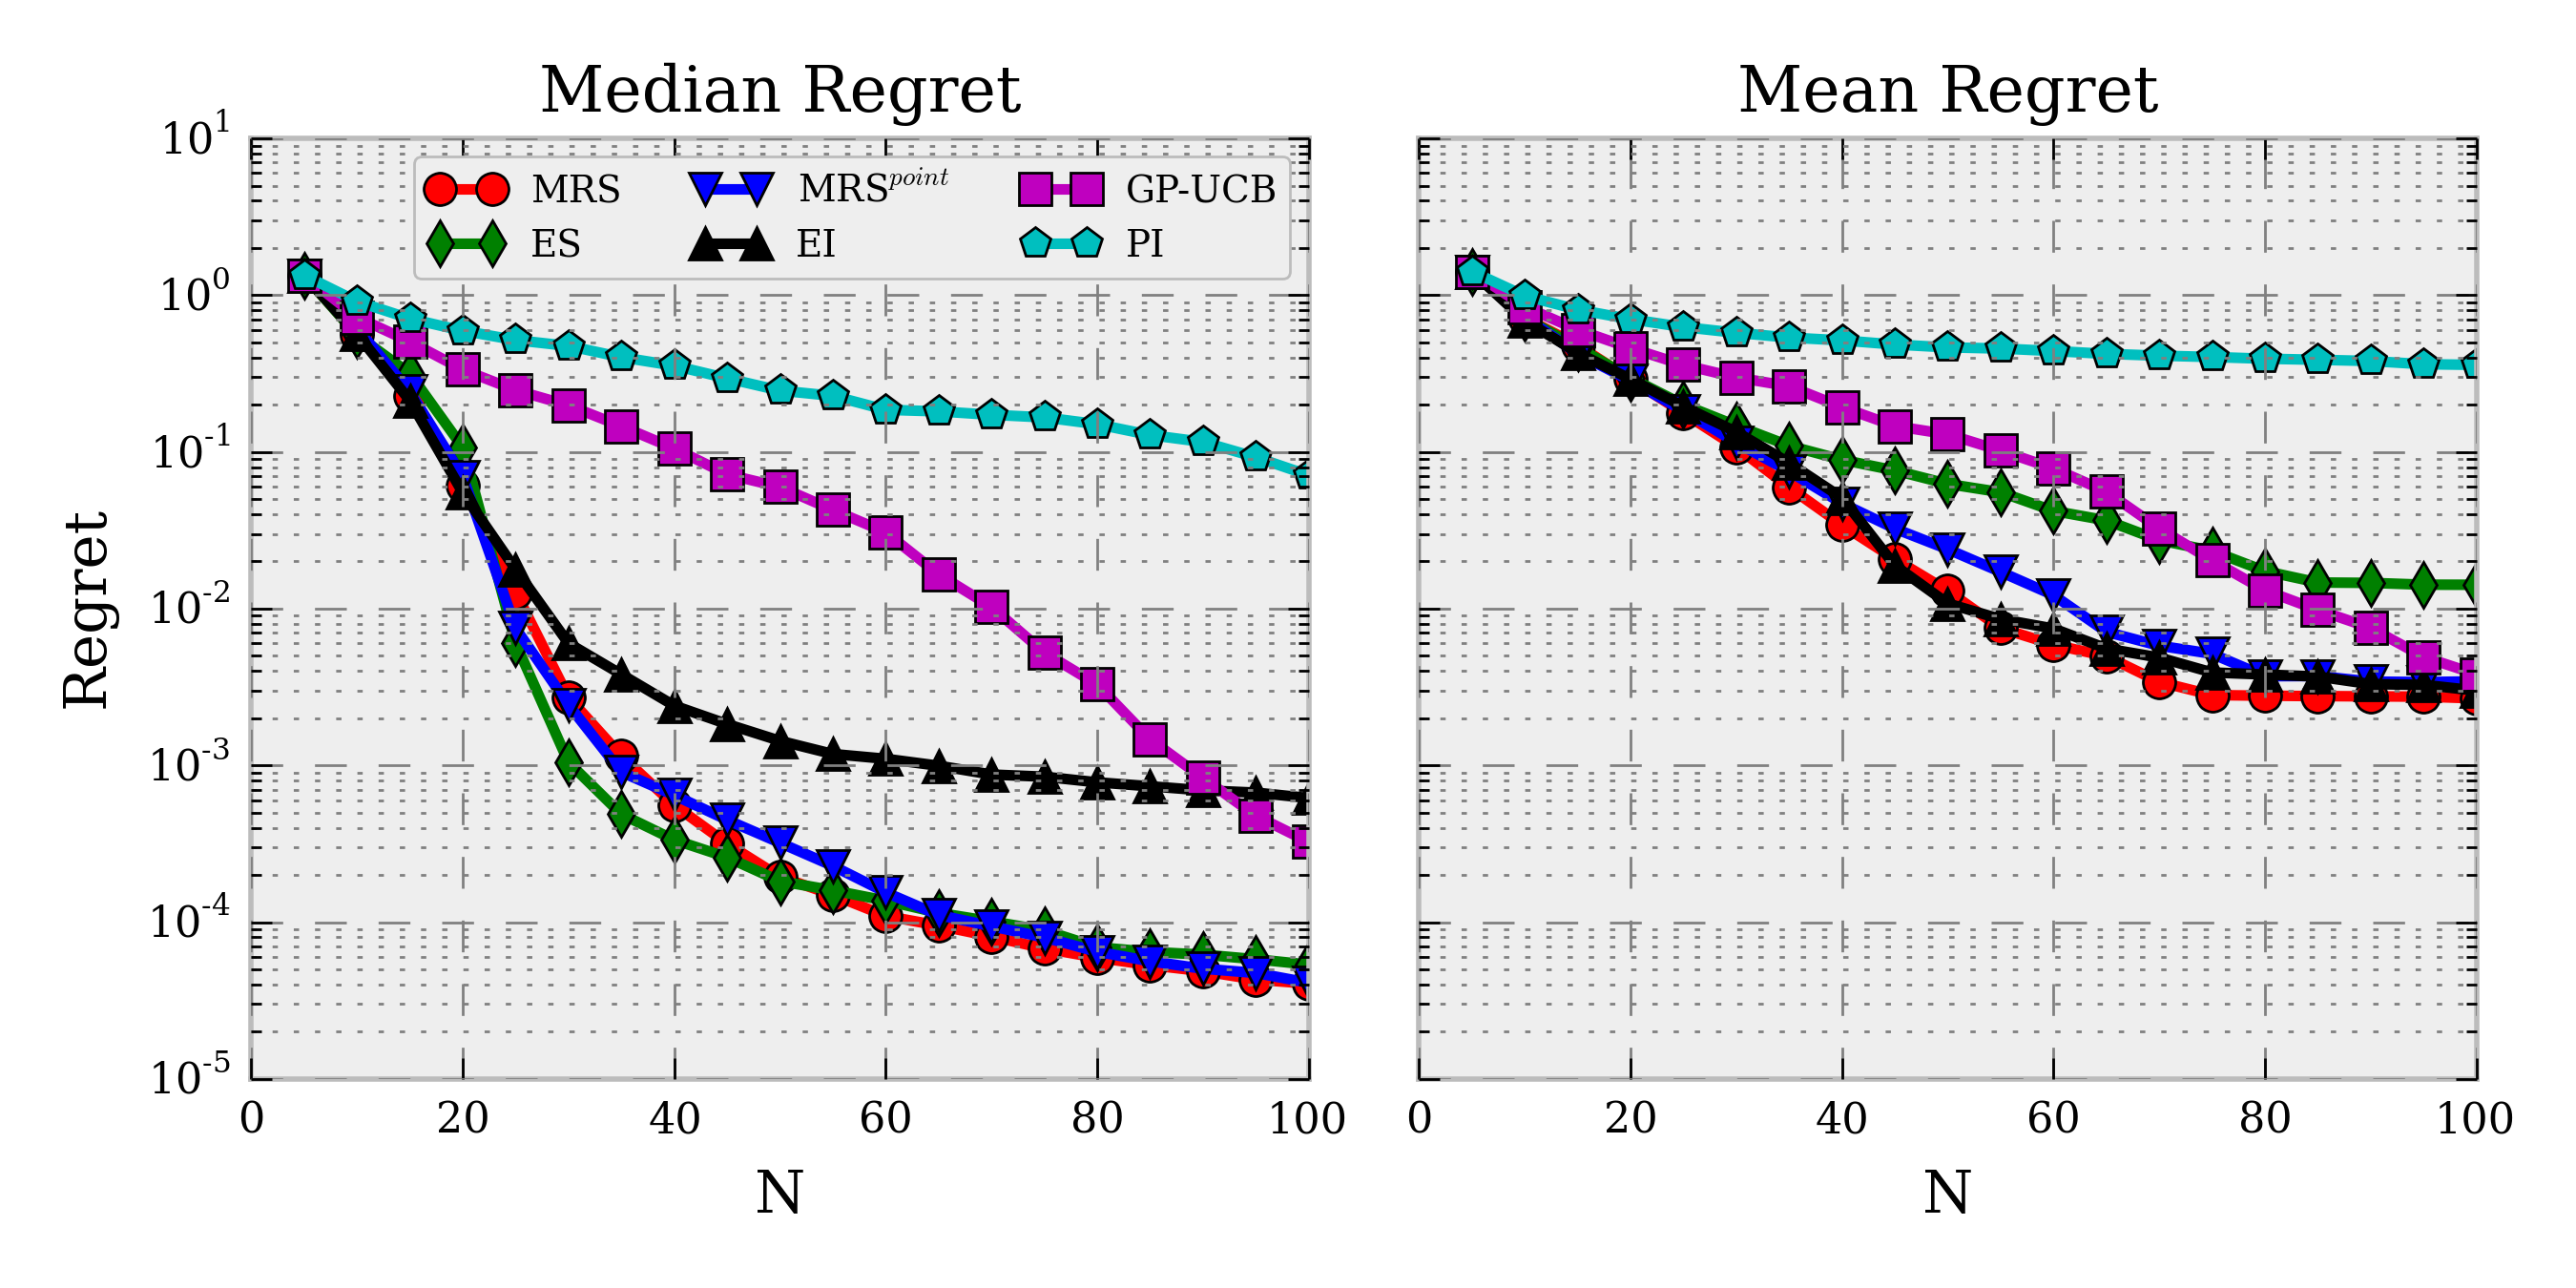
\includegraphics[width=.9\columnwidth]{../pics/empirical_comparison} \\
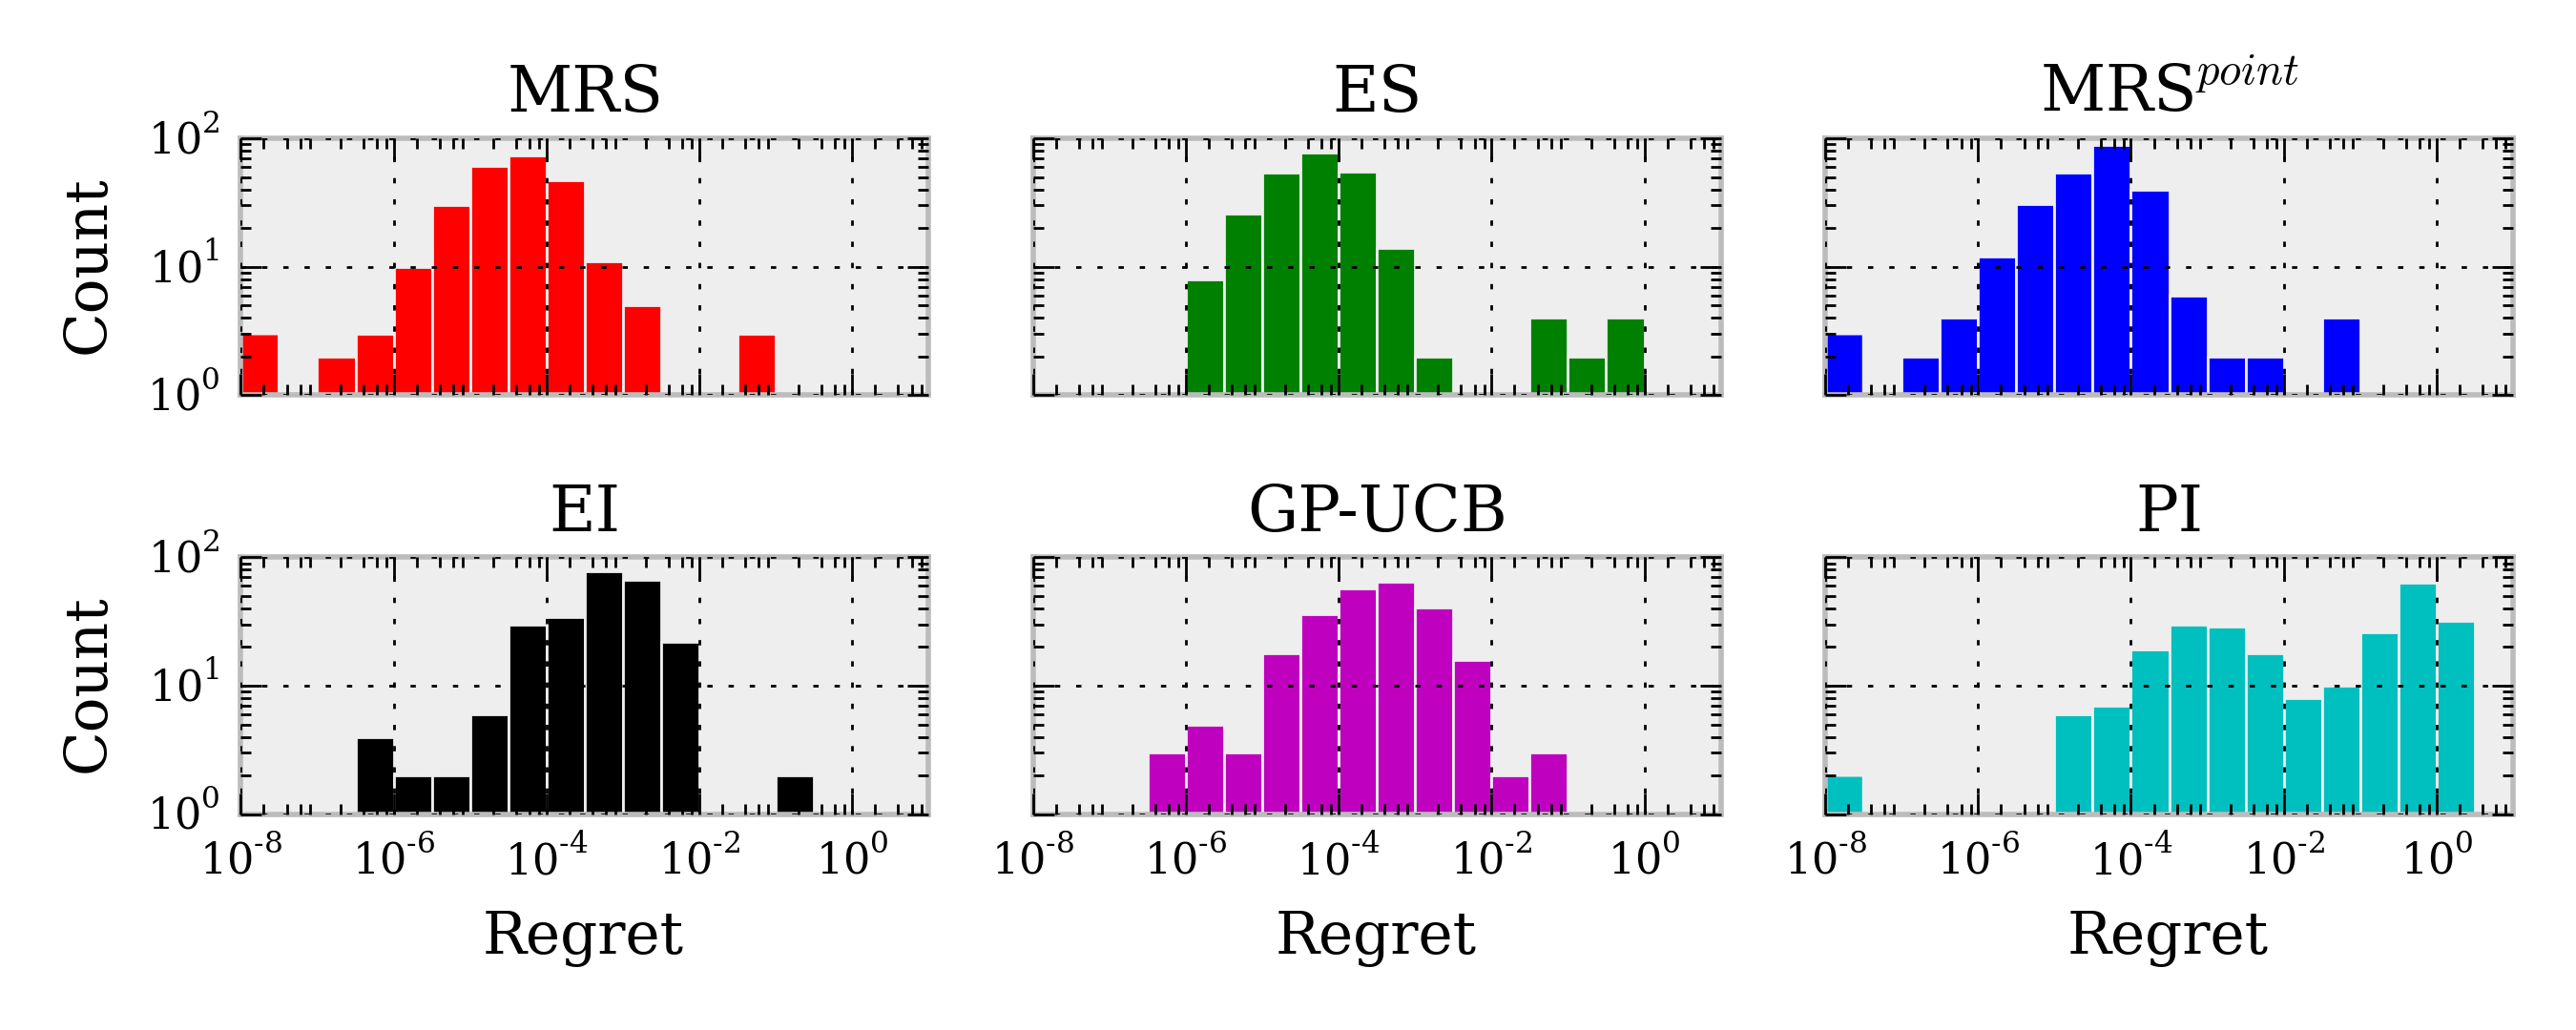
\includegraphics[width=.9\columnwidth]{../pics/hist}
\caption{(Top) Median and mean simple regret over $250$ repetitions for different acquisition functions. Shown is the simple regret of the recommendation $\mathbf{\tilde x}_N$ after $N$ trials, i.e., the point which maximizes the GP posterior
mean. (Bottom) Histogram of the simple regret after performing $N=100$ trials for different acquisition functions (note the log-scales).}
\label{fig:empirical_comparison}
\end{figure}


\begin{figure}
\centering
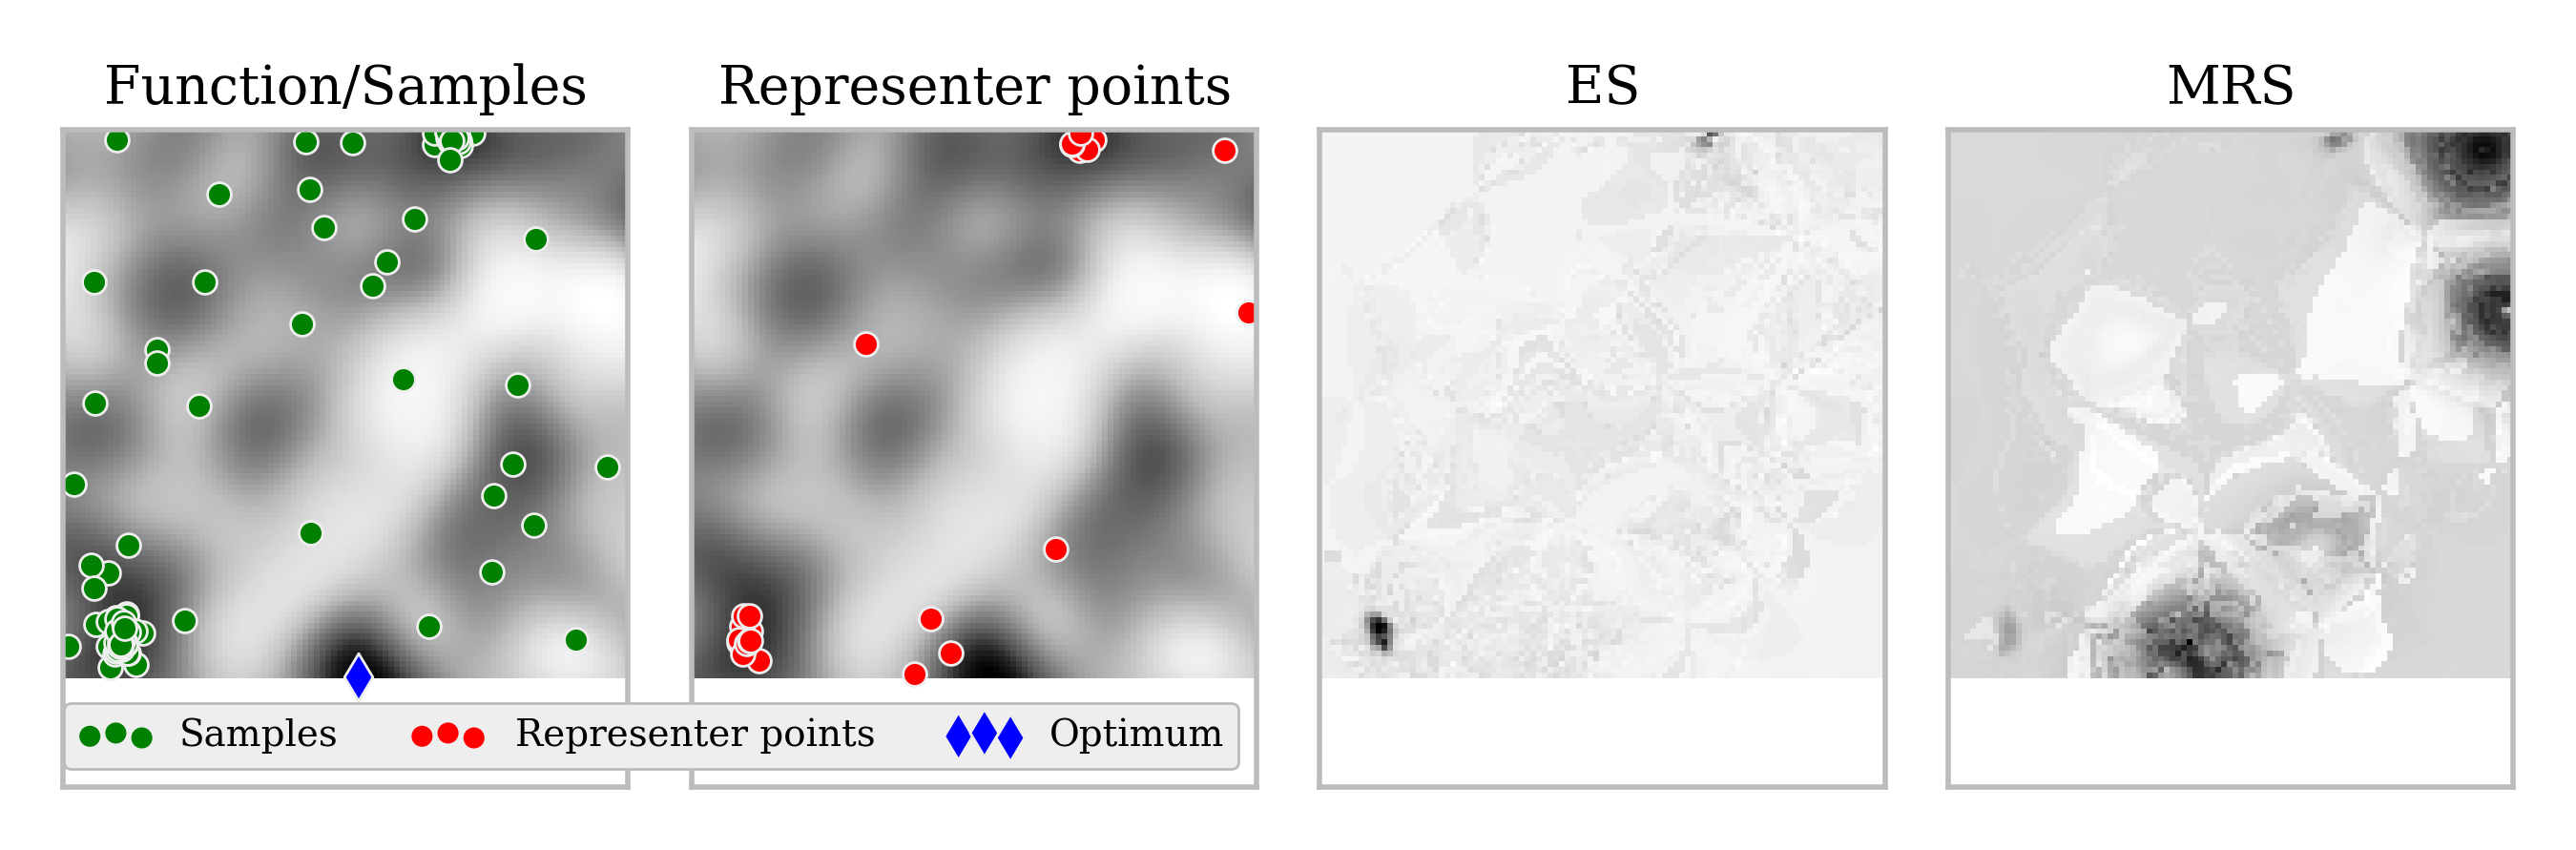
\includegraphics[width=.9\textwidth]{../pics/es_analysis}
\caption{Illustration of acquisition functions on a target function for
100 given samples and 25 representer points; darker areas correspond to larger values. ES focuses on sampling in areas with high density of $p^\star$ (many representer points), while MRS focuses on unexplored areas that are populated by representer points (non-zero $p^\star$).
}
\label{fig:es_analysis}
\end{figure}

\end{center}
\end{block}

\begin{block}{\blocktitle{Outlook}}
\begin{itemize}
 \item Comparison to other active task (context) selection approaches \cite{fabisch_accounting_2015}
 \item Scaling up to higher dimensions using approaches such as REMBO
\cite{wang_bayesian_2013}
 \item Evaluation on real systems and related tasks such as robotic locomotion \cite{calandra_bayesian_2014,lizotte_automatic_2007} and robot grasping \cite{kroemer_combining_2010}
 \item More information on project BesMan (Behaviors for Mobile Manipulation):
\url{http://robotik.dfki-bremen.de/en/research/projects/besman.html}
\end{itemize}
\end{block}

\begin{block}{\blocktitle{References}}

\begin{multicols}{2}
{\scriptsize
\setbeamertemplate{bibliography item}[text]
\bibliographystyle{abbrv}
\bibliography{../literature}
}
\end{multicols}

\end{block}
